\documentclass[../../main]{subfiles}
\begin{document}
% Dataset synthetization (mostrare i dieci step che hanno portato al dataset su cui è stato fatto il training)

\label{ss:dataset-synthetization}
\subsection{Dataset synthetization}
We started from geolife, a great dataset for our purpose because it collects a huge number of trajectories from a lot of user. What we want to learn is which place category will fit the user situation, by using his time \& human activity \& position.
To achieve this goal we first need to preprocess the dataset.

\paragraph{Stay Point}
Our goal is to recommend some \textbf{place} where a user spend a certain amount of time. We trasleted this as the centroid
of a trajectory included in a certain interval of time and space. We take inspiration from the paper 
\textit{``Collaborative Location and Activity Recommendation with GPS History Data''}. 
We use a distance threshold of 100 meters and a time threshold of 5 minutes to find a staypoint in a trajectory.
\begin{figure}[h]
    \centering
    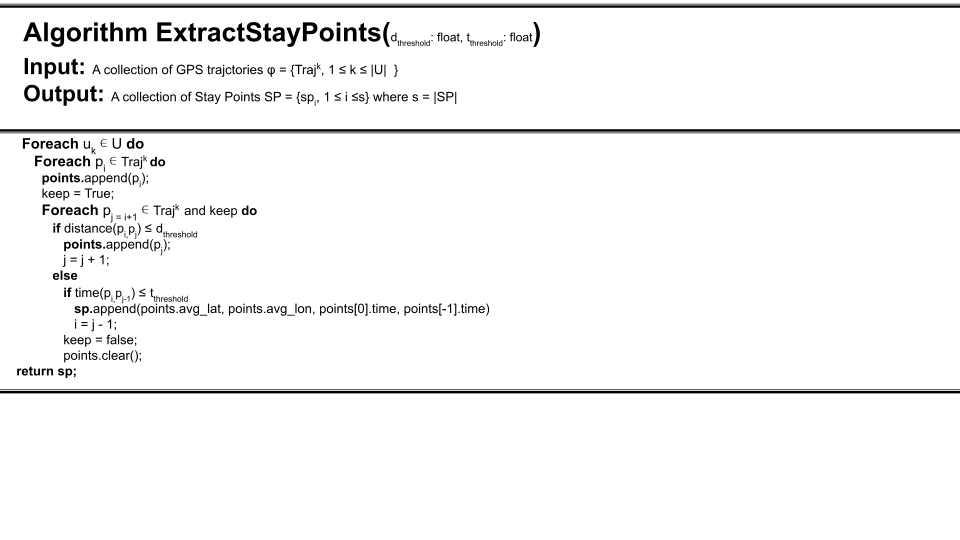
\includegraphics{images/sp.png}
    \caption{Stay point Extraction algorithm}\label{fig:extraction_sp}
\end{figure}

\paragraph{Cluster}
From the staypoint extracted we generated the clusters by using DBscan and as eps (maximum distance between two points to be considered neighbor) 
300 meters because we think that a stay point should work in a radius of 300 meters. Then we used the clustered stay points to ask Place APIs, from Google, 
which categories of business activty were found, we save the nearest one and we use as time for that activity the quantile of the time of arrival in UTC format.
We had to cluster the stay points because Place API is not free and the sp we found were really a lot. Probably with a free API we could train a more precise model.
\paragraph{Human activity}
Because we can't know which activity were doing the users in that SP, since it is created from a lot of sp of the users, we generated it randomly 
because an average of all was less meaning. We thought that a restaurant should be recommended when the user is walking or is still, because
the most frequently situation when a user need to find some place to eat is when he do some walking activity, like visiting the city center.
Instead for sport or leisure we generated also activity as car, bus or bike besides walk and still. The main thought was that when a user is moving with 
some transport he is going to hang out and want to have fun or maybe is going in same green space to take a walk or run.

By doing this we generated a dataset with clustered stay point were we can infer, thanks to a Decision Tree, which place should be recommended by 
receiving as input the user position, his human activity and the actual time.

\end{document}